\documentclass[8pt]{article}
\usepackage{graphicx,psfrag,url}
\usepackage{amssymb,amsmath}
\usepackage{subfig}
\usepackage{fullpage}
\usepackage{appendix}
\usepackage{enumitem}% http://ctan.org/pkg/enumitem
\usepackage{multicol}% http://ctan.org/pkg/multicol
\usepackage{caption}
%\usepackage{cite}
\usepackage{microtype}
\usepackage{color}
\usepackage{tikz}
\usepackage{numcompress}
\DeclareGraphicsExtensions{.pdf,.png,.jpg}
\newcommand*{\boxedcolor}{red}
\makeatletter
\allowdisplaybreaks
\renewcommand{\boxed}[1]{\textcolor{\boxedcolor}{%
  \fbox{\normalcolor\m@th$\displaystyle#1$}}}
\makeatother
\newcommand{\BEAS}{\begin{eqnarray*}}
\newcommand{\EEAS}{\end{eqnarray*}}
\newcommand{\BEQ}{\begin{equation}}
\newcommand{\EEQ}{\end{equation}}
\newcommand{\BIT}{\begin{itemize}}
\newcommand{\EIT}{\end{itemize}}

\newcommand{\eg}{{\it e.g.}}
\newcommand{\ie}{{\it i.e.}}

\newcommand{\ones}{\mathbf 1}
\newcommand{\reals}{{\mbox{\bf R}}}
\newcommand{\integers}{{\mbox{\bf Z}}}
\newcommand{\symm}{{\mbox{\bf S}}}  % symmetric matrices

\newcommand{\nullspace}{{\mathcal N}}
\newcommand{\range}{{\mathcal R}}
\newcommand{\Rank}{\mathop{\bf Rank}}
\newcommand{\Tr}{\mathop{\bf Tr}}
\newcommand{\diag}{\mathop{\bf diag}}
\newcommand{\lambdamax}{{\lambda_{\rm max}}}
\newcommand{\lambdamin}{\lambda_{\rm min}}

\newcommand{\Expect}{\mathop{\bf E{}}}
\newcommand{\Prob}{\mathop{\bf Prob}}
\newcommand{\Co}{{\mathop {\bf Co}}} % convex hull
\newcommand{\dist}{\mathop{\bf dist{}}}
\newcommand{\argmin}{\mathop{\rm argmin}}
\newcommand{\argmax}{\mathop{\rm argmax}}
\newcommand{\epi}{\mathop{\bf epi}} % epigraph
\newcommand{\Vol}{\mathop{\bf vol}}
\newcommand{\dom}{\mathop{\bf dom}} % domain
\newcommand{\intr}{\mathop{\bf int}}

\newcommand{\sign}{\mathop{\bf sign}}
\newcommand{\devices}{\mathcal{D}}
\newcommand{\terminals}{\mathcal{T}}
\newcommand{\nets}{\mathcal{N}}
\newcommand{\AC}{\mathcal{T}^\mathrm{ac}}
\newcommand{\DC}{\mathcal{T}^\mathrm{dc}}
\DeclareMathOperator*{\cart}{\times}

%\usepackage{circuitikz}
%\DeclareMathOperator*{\mathbf{prox}}{prox}
%\DeclareMathOperator*{\argmin}{argmin}
%\usepackage[small,bf]{caption}
%\usepackage[small,bf]{caption}
%\setlength{\captionmargin}{30pt}
\bibliographystyle{alpha}
\begin{document}

\title{
	\textbf{Response letter to Reviewers' Feedback for ``Look-Ahead SCOPF (LASCOPF) for Tracking Demand Variation via Auxiliary Proximal Message Passing (APMP) Algorithm"}\\\vspace{5mm}\small{\textbf{Sambuddha Chakrabarti \& Ross Baldick}}
}
\maketitle
\noindent\author{}
%-----------------------------------------------------------------------------------------------------------------------------------------
\vspace*{-10mm}
\section{Comment from the Editor}
\noindent\textbf{Reviewers find the present work interesting.  At the same time, they raise numerous areas that require further clarification and revision.  Please address these concerns in point wise fashion and indicate changes made to the manuscript to facilitate the review process. }\\

We highly appreciate the reviewing and coordinating efforts of the reviewers and the editor, respectively and are immensely thankful for the comments, questions, suggestions, and constructive criticisms. We are highly confident, that, because of these, the quality of our research and the presentation of the material, as it appears in the revised manuscript draft has significantly improved. We have put in our best efforts to follow the guidelines, attempted modifications of the draft according to the suggestions, and answered the questions, to the best of our knowledge. Please find below, the point-wise response to the reviewers' comments and also the appropriate changes that we have made to the paper manuscript draft.\\

\section{Response to Reviewer 1}
\noindent\textbf{General Comment: The paper proposes a bi-layer decomposition approach for look-ahead SCOPF.  The topic is interesting and the reviewer has the following comments/recommendations:}\\

Your words of appreciation are sincerely acknowledged by us. We thank you for that. Given below are our responses to your questions and suggestions.\\

\textbf{Question 1: Your have included base case 0 in contingency set in Section 3.1 but in the remaining part throughout you list the base case constraints separately, e.g., constraints (1b) and (1d), which are redundant regarding the previous definition. I suggest removing either the base case from contingency set or all redundant constraints.}\\

\textbf{Answer: }Thank you very much for your constructive suggestion. We have taken care of this issue in our revised manuscript draft. We have omitted the separate equations pertaining to the base-case with scenario superscript ``0" and combined them together with the ones pertaining to the contingency scenarios.\\

\textbf{Question 2: The notation especially the superscripts and subscripts is very heavy and makes the paper hard to read. For example, what does $P^{(2)}_{(1)}$ exactly mean in (2a)?}\\

\textbf{Answer: }Thank you very much, for pointing us to improve the explanation of the symbols used. We have expanded upon, provided more clarification, and also modified the explanation of the convention for symbols and especially that for variables in subsection 3.1 of the manuscript. In order to help the reviewer find our modified and updated explanation, we have written the text block in \textcolor{blue}{blue} ink. For the sake of integrity, we are repeating that block below:\\
\textcolor{blue}{The following is the convention we follow in order to identify the associations of any particular variable to the sets:\\ $\Big(x_{d(p_1)(p_2)}^{(p_3)(p_4)}\Big)^{(\nu)}$.\\In the above, $x_d$ is a variable associated with a device-terminal or node/net-terminal, $d$. ${(p_1)(p_2)}$ and ${(p_3)(p_4)}$ indicate the computational units/agents, denoted, respectively, by a combination of $p_1, p_2$ and $p_3, p_4$, where a particular $p_i$ may refer to either a dispatch interval or contingency scenario it is associated with. In this particular case, $p_2$ and $p_3$ might indicate, respectively, a contingency scenario and a dispatch interval. Together, the combination ${(p_1)(p_2)}$ denotes a particular computational agent linked to this particular combination. The above notation should be interpreted as the belief about the value of the variable, $x_d$ associated or linked to the superscripted computational agent (${(p_3)(p_4)}$), as held by the subscripted computational agent (${(p_1)(p_2)}$) at the $\nu^{-\text{th}}$ iteration. Let's take a look at the next example, to make the meaning clearer.\\ $\Big(P_{{N}_{t}(c_1)(\tau_1)}^{(c_2)(\tau_2)}\Big)^{(\nu)}$.\\The foregoing notation refers to the belief of the value of a variable $P_{N_t}$ associated with a particular terminal, $N_t$, (which is indexed by the $t$) of either a net or a device for the contingency scenario indexed by $c_2$ during $\tau_2$, as estimated by a computational agent linked to $\tau_1$ and contingency scenario, $c_1$. Sometimes we will use the net number instead of the terminal number in the above convention, when we want to indicate several devices connected to a particular net. If it is part of an iterative algorithm, then the outermost superscript $\nu$ indicates the iteration count. Whenever a variable is boldface, one or more of the indices will be missing and that means the boldface variable is a vector each of whose components will have all or some of the missing indices (the components themselves can be vectors or scalars). When the variable is not bold-face and still some of the indices are missing, that means it is a scalar and the missing indices are either irrelevant or their values are implied from the context. Also it is to be observed that since generators and loads are single terminal devices, it is not necessary to specify the terminals for these, unless absolutely required.}\\
As a general rule, (as mentioned in the explanation above) the numbers appearing within the parentheses in the subscript refer to the computing units or agents (associated with a scenario and/or a dispatch interval) holding a belief about the variable associated with the parenthesized numbers appearing in the superscript. In the particular case of equation (2a) mentioned in your question, $P_{(1)}^{(2)}$ therefore means what the computational agent linked to dispatch interval 1 thinks about the value of power in interval 2. \\

\textbf{Question 3: The necessity and merit of temporal decomposition in Section 4 needs to be clarified. It seems completely OK for each device to solve a small scale LASCOPF subproblem.}\\

\textbf{Answer: }We thank the reviewers for this question. We think this is a very good and important question. There are two main reasons for the temporal decomposition (even though, in principle, each device could solve a small scale LASCOPF). They are as follows:\\
\begin{enumerate}
    \item First of all, the temporal decomposition (and even scenario decomposition for the SCOPF, about which, we briefly mentioned in the simulation section, as well as post-contingency scenario decomposition, in case we are interested in solving $(N-1-1)$ SCOPFs) makes the theoretical analysis much more modular and helps greatly in coding and developing the software. With this approach, once we have developed the software module for the OPF (which is much easier to code, debug, implement, prototype, and attain convergence), we can subsequently reuse it in all the other above-mentioned problem classes with minimum or no change. 
    \item According to our experience, attaining convergence for SCOPF and beyond has been extremely hard (and often impossible) using just ADMM-PMP for most of the cases, beyond the simple two or three bus systems. Invoking the temporal decomposition and using APP as the outer layer of iteration, helps us achieve convergence and solve the problems very easily.
\end{enumerate}

\textbf{Question 4: It is stated in the paper that CVXGEN is more efficient than GUROBI. But from the official introduction one of the limitation is that CVXGEN does not work well for large problems. Can you perform further tests on a larger system?\\http://www.cvxgen.com/docs/index.html}\\

\textbf{Answer: }This is an excellent question. This issue is a conceptual one and we thank the reviewer for asking this. Even though it is true that CVXGEN generated custom solvers do not work well for large problems (in fact, it cannot generate solvers for large problem, in the very first place), however, in our bi-layered distributed APMP algorithm to solve $(N-1)$ LASCOPF problems, we have used the CVXGEN generated custom solvers only in order to solve the optimization sub-problems for each individual generator, which indeed are, small optimization problems (at most 4 variables; one each for real power generation in the current, previous, and next interval, and the fourth for voltage phase angle; and 6 constraints at most, consisting of those for generation limits and ramping limits; the number of variables and constraints are lesser for the terminal dispatch interval problems). Being custom solvers, CVXGEN solvers solve much faster as compared to GUROBI for solving the generator sub-problems. \\

\textbf{Question 5: In Table 3, why is ST of 14 Bus significantly larger than those of 30-, 48- and even 57-bus systems?}\\

\textbf{Answer: }We thank the reviewer for asking this excellent question. This is a very good observation, and reason for it to have taken so long for convergence for the 14 bus case is that, first of all, we have analyzed all the lines (20 in number) for contingency and secondly, we also suspect that this particular case is much more constrained (i.e. closer to the brink of infeasibility) than the other cases.\\

\textbf{Question 6: What is the tolerance of outer APP in Table 3?}\\

\textbf{Answer: }We thank the reviewer for asking for clarification. We have used the following value for the outermost APP iteration for table 3:\\
Final Tolerance $\epsilon_{\text{LASCOPF}}$: 0.6\\
We have also highlighted the relevant paragraph in the revised paper draft in \textcolor{blue}{blue} ink to easily attract attention of the reviewer to this statement.\\

\textbf{Question 7: It is often hard to reconcile the tolerances of inner and outer layers to balance accuracy and efficiency. How did you handle that? In Table 3, some cases converge using just 1 outer iteration. What is the unit in Table 3?}\\

\textbf{Answer: }We thank the reviewer for asking for clarification. We agree that it's very hard to reconcile the tolerances of inner and outer layers to balance accuracy and efficiency, and in our case, we needed to strike some compromise between the two. In our case, we repeat below, (from the revised paper draft, where we have marked the paragraphs in blue ink for the reviewer to spot easily) the different tolerances and means of tuning that we have used to attain reasonably accurate convergence within reasonable amount of time :\\
For the innermost OPF simulations, which we solve by using ADMM-PMP, we have used the primal and dual residual tolerances to be 0.06 and 0.6, respectively (the reason, we use a higher value for the dual residual is that, we have observed that we get accurate enough solution for even somewhat higher value of the dual residual) and we have used a discrete version of proportional+derivative controller to adjust the value of $\rho$ for the first 3000 iterations, such that at each iteration the relationship $\rho\times\epsilon_{primal}=\epsilon_{dual}$ is maintained, where $\epsilon_{primal}$ and $\epsilon_{dual}$ are respectively the primal and dual residuals. After the first 3000 iterations, if the algorithm hasn't still converged, then $\rho$ is held fixed at the last value. The initial value of $\rho$ at the beginning of the iterations is taken as 1. \iffalse We have shown in Figure \ref{ADMM-PMP300}, one typical plot for the first 70 iterations of the innermost ADMM-PMP iterations for the 300 bus case for contingency scenario:2 and dispatch interval:3. This set of ADMM-PMP iterations was executed for the last iteration of the outer APP layers, both for consensus among scenarios, as well as, among dispatch intervals.\fi The following are the APP parameters for outer iterations for attaining consensus among the different base/contingency scenarios for solving SCOPFs.
\begin{itemize}
    \item $\alpha_{\text{SCOPF}}=5$ for $\nu\leq5$, $\alpha_{\text{SCOPF}}=3$ for $5<\nu\leq10$, $\alpha_{\text{SCOPF}}=2.5$ for $10<\nu\leq15$, $\alpha_{\text{SCOPF}}=1.25$ for $15<\nu\leq20$, and $\alpha_{\text{SCOPF}}=0.5$ for $\nu>20$, $\beta_{\text{SCOPF}}=200$, $\gamma_{\text{SCOPF}}=100$ ($\nu$ is the APP iteration count)
    \item Final Tolerance $\epsilon_{\text{SCOPF}}$: 0.7
\end{itemize}
Following are the APP parameters for outermost iterations for attaining consensus among the different MW outputs in different intervals, limited by ramp-rate constraints.
\begin{itemize}
    \item $\alpha_{\text{LASCOPF}}=10$ for $\mu_{APP}\leq5$, $\alpha_{\text{LASCOPF}}=5$ for $5<\mu_{APP}\leq10$, $\alpha_{\text{LASCOPF}}=2.5$ for $10<\mu_{APP}\leq15$, $\alpha_{\text{LASCOPF}}=1.25$ for $15<\mu_{APP}\leq20$, and $\alpha_{\text{LASCOPF}}=0.5$ for $\mu_{APP}>20$, $\beta_{\text{LASCOPF}}=200$, $\gamma_{\text{LASCOPF}}=100$ ($\mu_{APP}$ is the outermost APP iteration count)
    \item Final Tolerance $\epsilon_{\text{LASCOPF}}$: 0.6
\end{itemize}
As can be seen, for both the inner and outer APP iterations, we have used changing step-length. The way we chose those values are ad-hoc and gives a reasonable balance between accuracy and solve-time.\\

With the particular loading condition and since we used a certain kind of warm start (i.e. as our initial guess for the power generations for outer APP layer, we used the known dispatch values from the previous interval), it did happen that a couple cases converged with just one iteration. The unit is in MW (since we are measuring the power generation disagreements as our convergence metric).\\

\textbf{Question 8: How is the convergence metric calculated in inner iteration?}\\

\textbf{Answer: }Thank you very much, for asking this question. We have added paragraphs in the revised draft, explaining the calculation in \textcolor{blue}{blue} and are repeating here, foe the sake of completeness. In the innermost ADMM-PMP iterations, the convergence criteria is calculated as follows:\\
\textcolor{blue}{\textbf{Stopping criterion for ADMM-PMP: }We can define primal and dual residuals ${\mathbf{r}}^{(\nu)}\in\mathbb{R}^{|\mathcal{N}|+|\mathcal{T}|}$ and ${\mathbf{s}}^{(\nu)}\in\mathbb{R}^{|\mathcal{N}|+|\mathcal{T}|}$, respectively (at the end of ADMM-PMP iteration $\nu$, for the
PMP algorithm as:
\[
{\mathbf{r}}^{(\nu)} = \left(\hat {\mathbf{P}}^{(\nu)}, \tilde{\mathbf{\Theta}}^{(\nu)}\right),
{\mathbf{s}}^{(\nu)} = \rho\left((({\mathbf{P}}^{(\nu)} - \mathbb{A}\times\hat {\mathbf{P}}^{(\nu)}) - ({\mathbf{P}}^{(\nu-1)} - \mathbb{A}\times\hat {\mathbf{P}}^{(\nu-1)})), (\hat {\mathbf{\Theta}}^{(\nu)}- \hat {\mathbf{\Theta}}^{(\nu-1)})\right).
\]
Where \begin{itemize}
    \item $\mathbb{A}\in\mathbb{R}^{|\mathcal{T}|\times|\mathcal{N}|}$ is the terminal to node incidence matrix, with 
    \begin{itemize}
        \item $\mathbb{A}(t_k,N_i)=1$ if terminal $t_k$ is connected to node $N_i$
        \item otherwise, $\mathbb{A}(t_k,N_i)=0$
    \end{itemize}
    \item ${\mathbf{P}}^{(\nu)}\in\mathbb{R}^{|\mathcal{T}|}$ is a vector of the real power iterates of all the devices-terminals (generators, transmission lines, and loads) connected to a particular node, at the end of the $\nu^{\text{-th}}$ ADMM-PMP iteration.
    \item ${\hat{\mathbf{P}}}^{(\nu)}\in\mathbb{R}^{|\mathcal{N}|}$ is a vector of the real power nodal average injections (i.e. real power iterates of all the devices (generators, transmission lines, and loads) connected to a particular node, divided by the number of devices) at the end of the $\nu^{\text{-th}}$ ADMM-PMP iteration.
    \item $\tilde{\mathbf{\Theta}}^{(\nu)}\in\mathbb{R}^{|\mathcal{T}|}$ is the difference between the voltage phase angle iterate of each device, connected to a particular node and the average voltage phase angle at the node, at the end of the $\nu^{\text{-th}}$ ADMM-PMP iteration.
    \item ${\hat{\mathbf{\Theta}}}^{(\nu)}\in\mathbb{R}^{|\mathcal{N}|}$ is a vector of the voltage phase angle nodal average (i.e. voltage phase angle iterates of all the devices (generators, transmission lines, and loads) connected to a particular node, divided by the number of devices) at the end of the $\nu^{\text{-th}}$ ADMM-PMP iteration.
\end{itemize}
A simple terminating criterion for prox-project message passing is when
\[
\| {\mathbf{r}}^{(\nu)} \|_2 \leq \epsilon^\mathrm{pri}, \qquad \|{\mathbf{s}}^{(\nu)}\|_2 \leq \epsilon^\mathrm{dual},
\]
where $\epsilon^\mathrm{pri}$ and $\epsilon^\mathrm{dual}$ are,
respectively, primal and dual tolerances and the norms are second norms.}\\

\textbf{Question 9: Have you compared you results (both optimal solution and objective value) with benchmark obtained by the centralized method?}\\

\textbf{Answer: }We thank the reviewer for asking for the suggestion. We have provided a table and a short explanation at the end of section 2.2 for the benchmark comparison.\\

\textbf{Question 10: Since you mentioned SDP relaxation for OPF, some recent advance in SOCP relaxation [r1] and chordal relaxation [r2] along with their application in related distributed OPF [r3-r4] should also be discussed in Section 2.
\begin{itemize}
    \item [r1] M. Farivar and S. H. Low, "Branch Flow Model: Relaxations and Convexification (Part I)," IEEE Transactions on Power Systems, vol. 28, pp. 2554-2564, 2013.
    \item [r2]  S. H. Low, "Convex Relaxation of Optimal Power Flow, Part I: Formulations and Equivalence," IEEE Transactions on Control of Network Systems, vol. 1, pp. 15-27, 2014.
    \item [r3] E. Dall'Anese, Z. Hao, and G. B. Giannakis, "Distributed Optimal Power Flow for Smart Microgrids," IEEE Transactions on Smart Grid, vol. 4, pp. 1464-1475, 2013.
    \item [r4] W. Zheng, W. Wu, B. Zhang, H. Sun, and Y. Liu, "A Fully Distributed Reactive Power Optimization and Control Method for Active Distribution Networks," IEEE Transactions on Smart Grid, vol. 7, pp. 1021-1033, 2016.
\end{itemize}}

\textbf{Answer: }We thank the reviewer for this comment and pointing us towards good recent references. We have just added the suggested references in the bibliography of the revised draft and cited them in section 2 (marked in blue ink).\\

\textbf{Question 11: Convergence details of inner PMP iteration should be provided.}\\

\textbf{Answer: }Thank you for the suggestion. We have added figure describing the ADMM-PMP innermost convergence characteristics and also made mention of it in the revised paper draft (colored in blue ink), for the IEEE 300 bus system for contingency scenario:2 and dispatch interval:3 for the last iterations of the outer APP layers.\\



\section{Response to Reviewer 2}
\noindent\textbf{General Comment: The look-ahead SCOPF (LASCOPF) for tracking demand variation via auxiliary proximal message passing (APMP) algorithm is proposed in this manuscript and the case study is implanted to verify the effectiveness of the method. The method is effective for solving the problem. But the paper is not clear enough in some places, several issues should be clarified/justified before the manuscript should be considered suitable for publication.}\\

We are thankful to the reviewer, for reading our manuscript draft and providing us helpful suggestions and feedback. We have tried to follow the suggestions and modify our draft accordingly as best as we could. Given below are our specific responses\\

\textbf{Question 1: In section 2, the author summarizes the current research status, but does not point out the shortcomings of the existing research and the areas to be improved, nor does it clarify the advanced aspects of this paper compared with the existing research. The reviewer suggested that the author improve this.}\\

\textbf{Answer: }We want to express our thanks to reviewers for the suggestion. We have included a subsection within section 2, detailing the specific contributions of the present work in blue ink. We are repeating it here, for the sake of easy reference and integrity. \\
While there has been some excellent work in the recent past on $(N-1)$ and $(N-k)$ SCOPFs as evidenced by references \cite{capitanescu2011state, lubin2015robust, amjady2011security, la1998line, articleSCOPF}, however, there is a dearth of literature on multiple-dispatch interval SCOPF. Also, a vast majority of the academic literature present till date on the topic of SCOPF either solve a corrective control version of the SCOPF (by changing generator dispatch to relieve line congestion in the outaged cases) or they solve a chance constrained version. Moreover, in the academic body of literature, there is also a severe lack of materials, describing the software implementation for SCOPF and LASCOPF for the preventive control version. The main contribution of our work, in the light of the above, can be summarized as presenting the preventive control version of $(N-1)$ SCOPF for multiple dispatch intervals, as a part of which, we have also developed a software for implementing the mathematical model and the algorithms, which utilizes a two-layered distributed algorithm.\\
 
\textbf{Question 2: The reviewer suggests that the author explain the specific meaning of each of Equations 1-4 after each set of equations.}\\

\textbf{Answer: }We want to express our thanks to the reviewer for the suggestion. We have included detailed explanations of the respective sets of equations (after each of them) and colored them in blue ink for easily spotting them.\\

\textbf{Question 3: The reviewer suggests that the author supplement the flow chart to show the specific process of the proposed algorithm more clearly.}\\

\textbf{Answer: }We want to express our thanks to the reviewer for the suggestion. We have included three flowcharts (each corresponding to, respectively, the outermost APP, the inner APP, and the innermost ADMM-PMP layers of the APMP algorithm to solve the LASCOPF problem), provided explanations of the program-flow shown in them (highlighted in the blue ink), and also established the connection between them, with each other.\\

\textbf{Question 4: In Figure 8, both the text and the legend are small, and the reviewer recommends that the author make adjustments.}\\

\textbf{Answer: } We want to thank the reviewer for pointing this out. We have, in the revised draft, enlarged the figure and the legends and texts to cover the entire page.\\
 
\textbf{Question 5: In this paper, the author proposes a new algorithm, and verifies the convergence and algorithm efficiency, but does not compare this algorithm with the traditional algorithm to prove its superiority. The reviewer suggests that the author set up a comparative study.}\\

\textbf{Answer: } We want to thank the reviewer for pointing this out. We have, devoted a subsection (in blue ink) in the revised draft, for the comparative study, drawing materials from two of our recently co-authored published papers.\\

\section{Response to Reviewer 3}

\noindent\textbf{General Comment: This paper introduces a hybrid algorithm for solving the Look-Ahead Security Constrained Optimal Power Flow (LASCOPF) problem, in which the load demand varies over dispatch intervals according to some forecast . The idea of the article is that the outer layer uses the Auxiliary Problem Principle (APP) for distributed computation across several dispatch intervals, and the inner layer uses Proximal Message Passing (PMP) for distributed computation within each of the dispatch interval across different devices, nodes or nets. The algorithm is a fully decentralized algorithm (without any central coordinator).}\\

We express our sincere gratitude to the reviewer, for reading our manuscript draft and summarizing it nicely. \\

\textbf{This paper mainly introduces a model and its application. Reviewers have the following questions:}\\

\textbf{Question 1: The table 1 of the numerical experiment shows the generator data for 5 bus system and only two sets of data are involved it, which needs more data to explain the situation.}\\

\textbf{Answer: } We thank the reviewer for this question. We want to clarify that the reason, there are two sets of data, or two rows of data, to be precise, is that, there are only two generators in the 5 bus system (refer to Figure \ref{5Bus}; here, the numbers appearing are the same, as appears in the corresponding tables in the paper manuscript, for the generator capacity, cost coefficients, load, and transmission line data). 
\begin{figure}
\begin{center}
%\hspace*{-2cm}
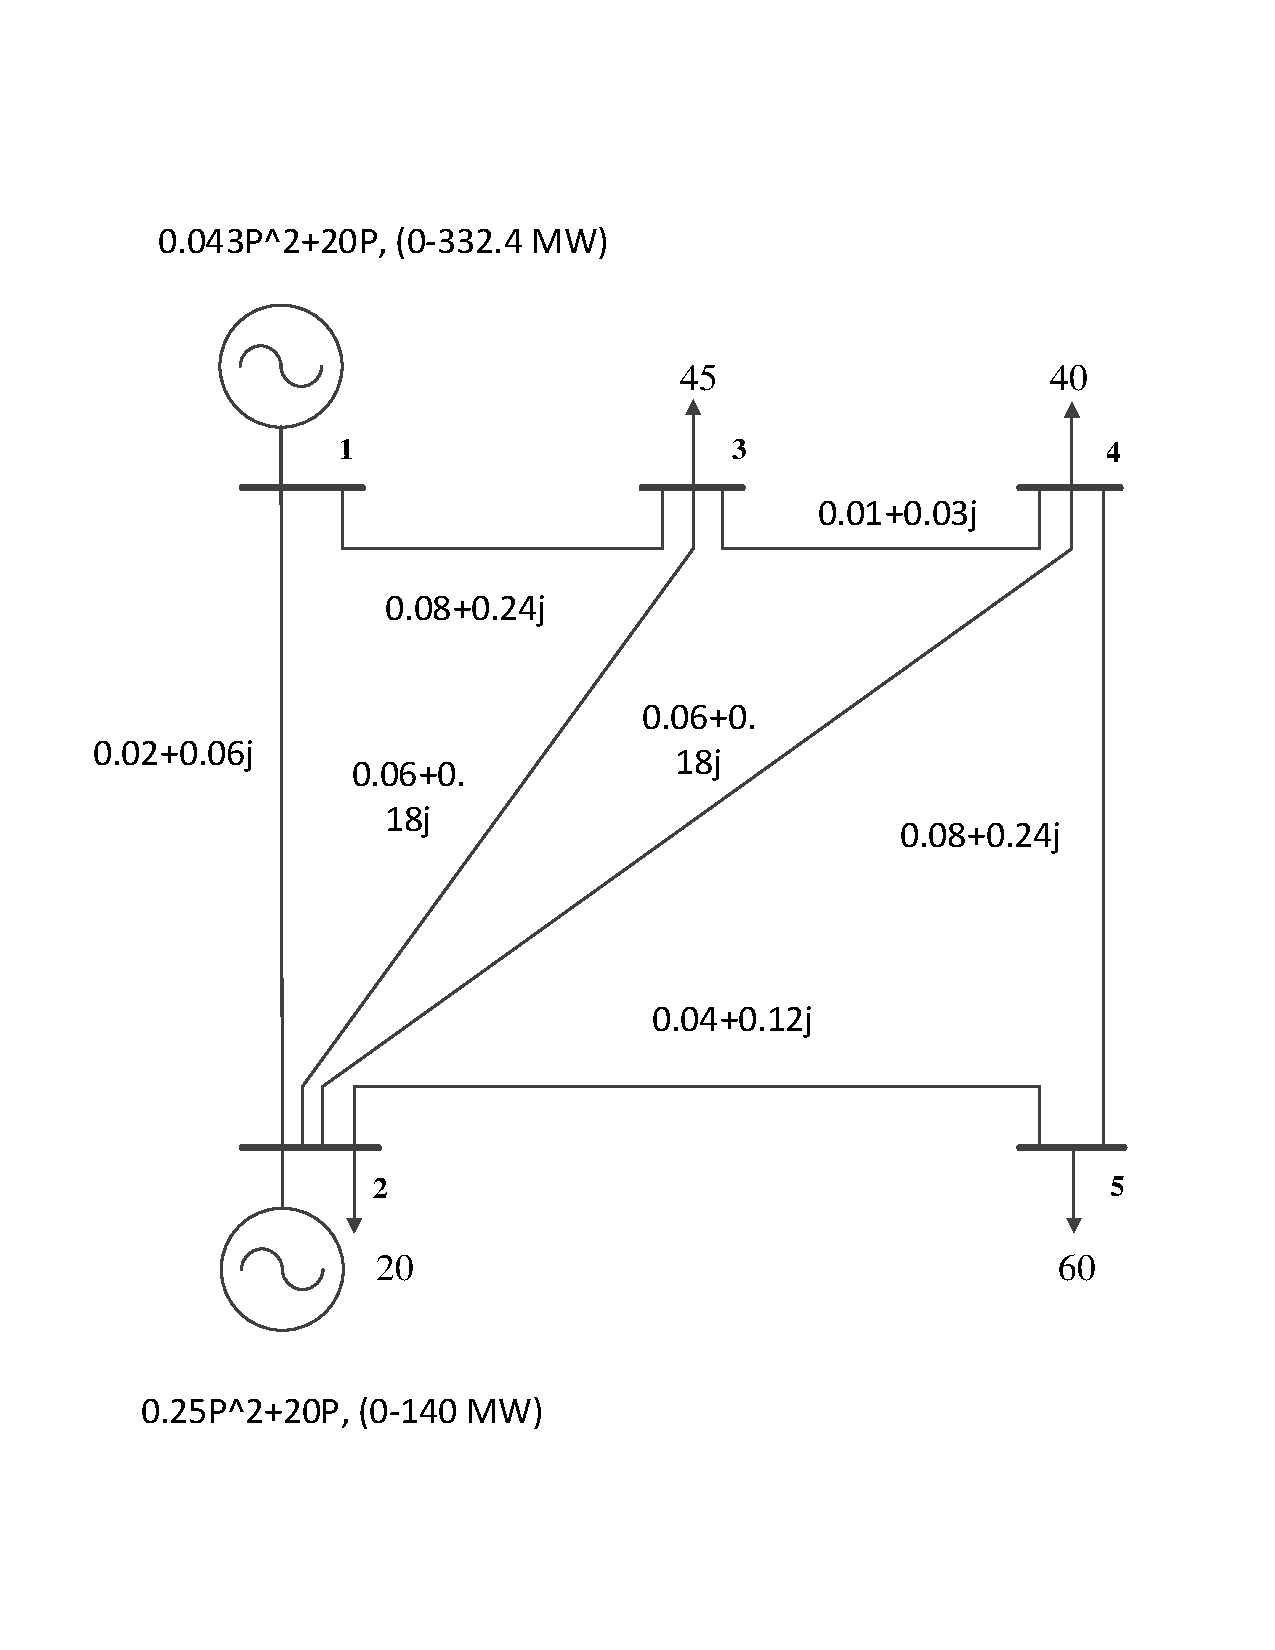
\includegraphics[height=12cm,width=15cm]{5_bus.pdf}
%\vspace*{-4cm}
\caption{5 Bus system schematic}
\label{5Bus}
\end{center}
\end{figure}
In the table, we have mentioned all the relevant details, along with the units. However, we would like to ask the reviewer to kindly provide us more specific details regarding what other missing data for what all quantities we need to provide. We will be happy to furnish any relevant data that the reviewer thinks is necessary and is missing. 

\textbf{Question 2: The decentralized algorithm mentioned in the article does not reflect its advantages in numerical experiments, and lacks contrast experimental data.}\\

\textbf{Answer: } We thank the reviewer for this question. We have added subsection 2.2 in section 2, to draw comparison with other algorithms, and point out the advantages/disadvantages of the current scheme.\\

\textbf{Question 3: The author needs to carefully check the various grammars, terms and formulas which are used in the article. Reviewers find the following problem:}\\
\textbf{\begin{enumerate}
    \item In the P4 symbol description, the element is expressed in the text:T:Elements of T, whether there is symbol reuse.\\
    \textnormal{\textbf{Answer: } We have modified the notation in \textcolor{blue}{blue} in the appropriate places in the notations section, to address this issue. We have, specifically, in the modified draft, in order to make a distinction, between the set of transmission lines and the elements of that set, used $\mathbb{T}$ as the set and as before, used $T$ as its elements.}\\
    \item There is a lack of explanation for some variable symbols used in the formula.\\
    \textnormal{\textbf{Answer: } Thanks for bringing it up to our notice. We have added the missing symbol explanation in \textcolor{blue}{blue} ink for the dual variables in the notations section and also modified parts of the write-up for better explanation.}
    \item In P7, an equation formula should not be separated by a picture.\\
    \textnormal{\textbf{Answer: } Thank you for bringing it to our attention. We have corrected it in the modified draft.}
    \item There are problems with the layout of the article's font, format and so on.\\
    \textnormal{\textbf{Answer: } We thank the reviewer for bringing it to our notice. We made repeated and our best attempts to make sure that we follow the margins and also we have used the standard recommended Elsevier journal preprint (or submission manuscript) LaTeX package to compose the draft and used the recommended settings therein. However, we would like to request the reviewer and/or the editor to kindly point out specific issues that we should fix in this regard.}
    \item The symbols expressed by the same meaning in Table 4-8 should be unified.\\
    \textnormal{\textbf{Answer: } We thank the reviewer for the comment and suggestion. We would like to clarify that tables 4 to 10 comprises part of the input data for the simulations and they show only those loads that are varied over the dispatch intervals for 5, 14, 30, 48, 57, 118, and 300 bus test cases, respectively. The numbers show the magnitude of change (along with the signs for increase/decrease) from the standard values (that appear in the IEEE test cases). The reason we kept the tables separate, instead of fusing them into one, is because of the ease of maintaining the decorum and layout of the paper. However, it isn't clear to us, what exactly is asked of us to do in this particular comment. We therefore ask the reviewer and/or the editor to kindly provide further specific details and explanation on this suggestion, regarding what exactly we should do.}
\end{enumerate}
}\\
%\bibliographystyle{elsarticle-num}
\bibliography{msg_pass_sec.bib}
\end{document}


